\chapter{Techniques for Using the Sliders}\label{a.tech}

\sect{Setting the sliders in the motor blocks}

It is difficult to set the sliders precisely so that, for example, both
motors run at the same speed. We can use the translation of the
event-actions pairs into an AESL textual program to improve the
precision.

\trickbox{By moving the sliders on the motor action blocks, you will see
that the target speeds of the motors (\p{moter.X.target}) jump by steps
of 50 in the range $-$500 to 500. By moving the sliders carefully, you
can set the speeds to any of these values.}

\Cref{fig.textcode} shows the program from
\cref{fig.likes-hates} (where the pet likes you and follows you around)
along with the text translation at the right of the VPL window. This
text is modified automatically as you move the sliders.

\begin{figure}[hbt]
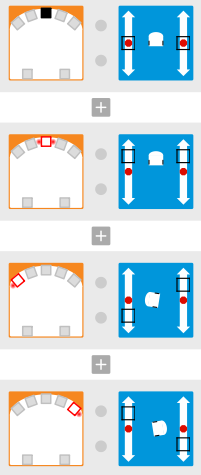
\includegraphics[width=0.3\textwidth]{likes}
\hfill
\begin{minipage}[b]{0.55\textwidth}
\begin{footnotesize}
\begin{verbatim}
onevent prox
    if prox.horizontal[2] < 1000 then
        motor.left.target = 0
        motor.right.target = 0
    end
    if prox.horizontal[2] > 2000 then
        motor.left.target = 300
        motor.right.target = 300
    end
    if prox.horizontal[0] > 2000 then
        motor.left.target = -300
        motor.right.target = 300
    end
    if prox.horizontal[4] > 2000 then
        motor.left.target = 300
        motor.right.target = -300
    end
\end{verbatim}
\end{footnotesize}
\vspace*{8ex}
\end{minipage}
\caption{A VPL program and the corresponding text program.}
\label{fig.textcode}
\end{figure}

\p{onevent prox} means: whenever the event of sampling the horizontal
sensors (the \emph{proximity} sensors, abbreviated \emph{prox})
occurs , the instructions on the following lines before \p{end} will be
run. The proximity event occurs 10 times a second.

When the event happens, the values of the sensors are checked using a
condition. Sensor number 2 (front center) is checked first:
\p{prox.horizontal[2]}. If this value is lower than 1000, the speeds of
the left and right motors are set to 0 using the instructions:

\begin{verbatim}
motor.left.target  = 0
motor.right.target = 0
\end{verbatim}

Every block \verb+if ... then ... end+ tests a specific sensor and runs
the associated instructions the result of test is true. The programs
runs the following algorithm:

\begin{enumerate}[start=0,noitemsep,nosep]
\item Tests if nothing is in front; if that is true, the robot stops.
\item Tests if something is in front; if that is true, the robot goes forward.
\item Tests if there is something at left; if that is true, the robot turns left.
\item Tests if there is something at right; if that is true, the robot turns right.
\end{enumerate}

Once all the sensors have been read and the appropriate action is
performed, the program waits for the next event \p{prox} and starts
these tests again. This happens again and again until the program is
stopped.

\sect{Setting the duration of the timer}

\trickbox{The duration in the time action block can be set in multiples of
one-quarter second (250 milliseconds) up to four seconds.}


\sect{Sensor event blocks in advanced mode}

This section describes features of the sensor event blocks that are
availble in advanced mode.

\subsection*{Setting the thresholds of the sensors}

In basic mode, the thresholds of the sensors are fixed. For the
horizontal sensors, a value above 2000 means that a lot of light is
reflected and an event will occur if the corresponding square is white,
while a value below 1000 means that little light is reflected and an
event will occur if the corresponding square is black. For the bottom
sensors, the values are 450 and 400.

In advanced mode, the thresholds can be set. The top slider sets the
threshold above which a white event occurs and the bottom slider sets
the threshold below which a black event
occurs:\label{p.proximity-sensitivity}

\begin{center}
\begin{tabular}{c@{\hspace{.1\textwidth}}c}
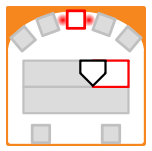
\includegraphics[width=.15\textwidth,keepaspectratio=true]{set-red}
&
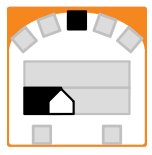
\includegraphics[width=.15\textwidth,keepaspectratio=true]{set-black}
\end{tabular}
\end{center}

\Cref{fig.follow-line-adv} shows the line-following program
(\cref{fig.follow-line-all}) in advanced mode. The sliders are set so that
the threshold is very low: 100 for both the upper and lower thresholds.

\begin{figure}
\subfigure[Start and stop the robot]%
{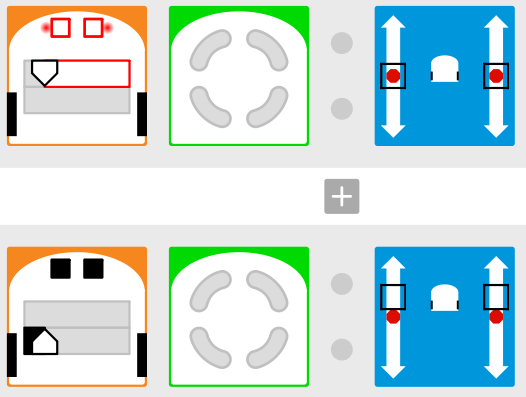
\includegraphics[width=0.45\textwidth]{line-forward-adv}}
\hfill
\subfigure[Correcting deviations]%
{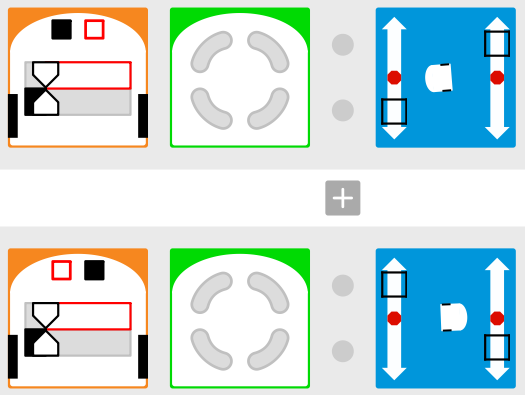
\includegraphics[width=0.45\textwidth]{line-controller-adv}}
\caption{A program for line following}
\label{fig.follow-line-adv}
\end{figure}

\subsection*{Multiple sensors}

If several sensors are set, they share the same thresholds:
\begin{center}
\begin{tabular}{c@{\hspace{.1\textwidth}}c}
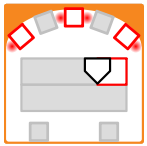
\includegraphics[width=.15\textwidth,keepaspectratio=true]{set-same}
&
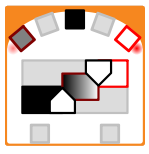
\includegraphics[width=.15\textwidth,keepaspectratio=true]{set-all}
\end{tabular}
\end{center}

\subsection*{Events for values between the thresholds}

There is an additional mode indicated by a dark gray
square:
\gr{set-gray}{.15}
In this mode, an event occurs if the value read by the read is greater
than the lower threshold (set by the lower slider) and less than the
upper threshold (set by the upper slider).
